\chapter{Jazyk ArchiMate}

Jazyk ArchiMate je jazykem pro modelování podnikové architektury. Jazyk je vyvíjen organizací The Open Group a je navržen tak, aby poskytoval jednotný jazkyk pro popis podnikové architektury. V práci je použita verze jazyka ArchiMate 3.2. Tento modelovcí jazyk byl zvolen na základě konzultace s vedoucím práce.

Jazyk je rozdělen na tři vrstvy, které je možné vidět na obrázku č. \ref{fig:archimate-core-framework} . První vrstvou je vrstva Obchodní, která zachycuje obchodní služby nabízené zákazníkům, které jsou v organizaci realizovány obchodními procesy vykonávannými obchoními aktéry. Druhou vrstvou je vrstva Aplikační, která popisuje aplikační služby, které podporují obchod, a aplikace, které je realizují. Třetí vrstvou je dvojvrstva Technologická \& fyzická, která zachycuje technologické služby, jako jsou služby zpracovávání, ukládání a komunikační služby potřebné ke spuštění aplikací, počítačový a komunikační hardware a systémový software, které tyto služby realizují. Součástí jsou fyzické prvky pro modelování fyzického vybavení, materiálů a distribučních sítí. \parencite{LanguageStructureArchiMate, OpenGroupStandard}

\begin{figure}[hbtp!]
  \centering
  \caption{Archimate Core Framework}
  \label{fig:archimate-core-framework}
  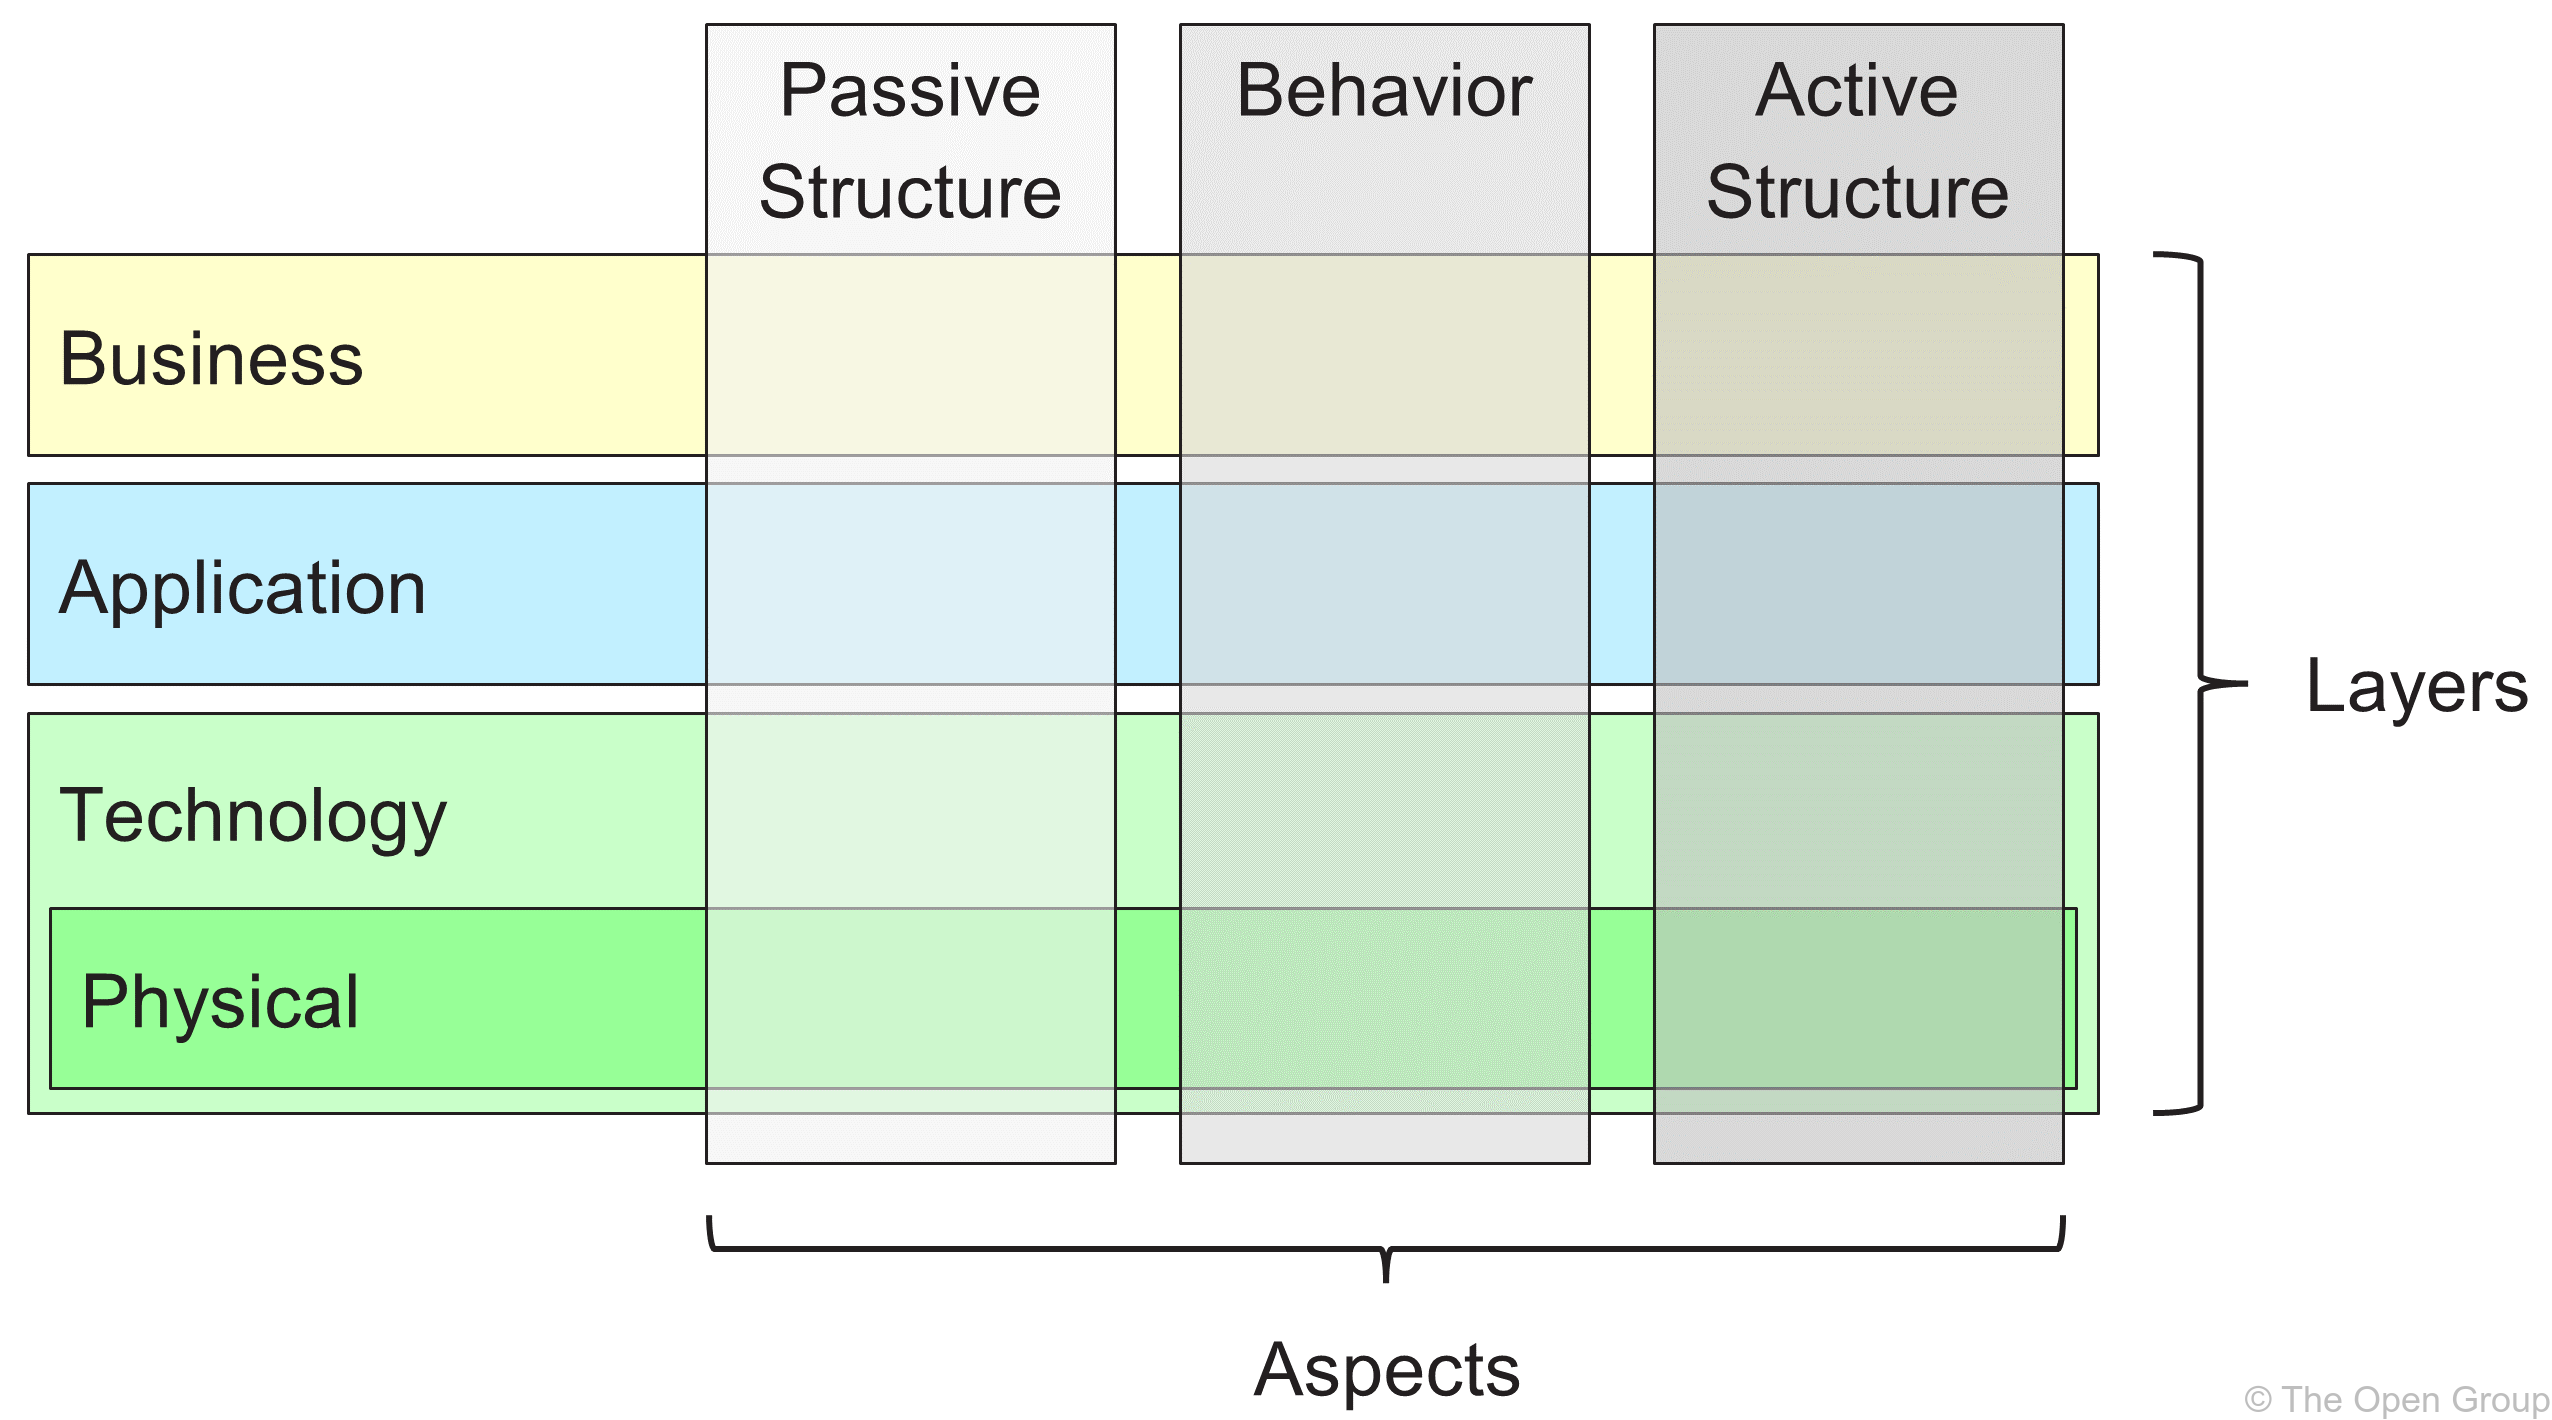
\includegraphics[width=0.8\textwidth]{img/fig-ArchiMate-Core-Framework}

  \scriptsize \textit{Zdroj:} Specifikace jazyka ArchiMate 3.2 \parencite{LanguageStructureArchiMate}
\end{figure}

\[TODO\]
Doplnit použité elementy

Elementy v jazyce ArchiMate jsou propojeny různými typy vztahů. Vztahy, které byly použity v této práci v kapitole č. \ref{chap:architektura} je možné vidět na obrázku č. \ref{fig:archimate-relationships}. 
\begin{figure}[hbtp!]
  \centering
  \caption{Vztahy v jazyce ArchiMate}
  \label{fig:archimate-relationships}
  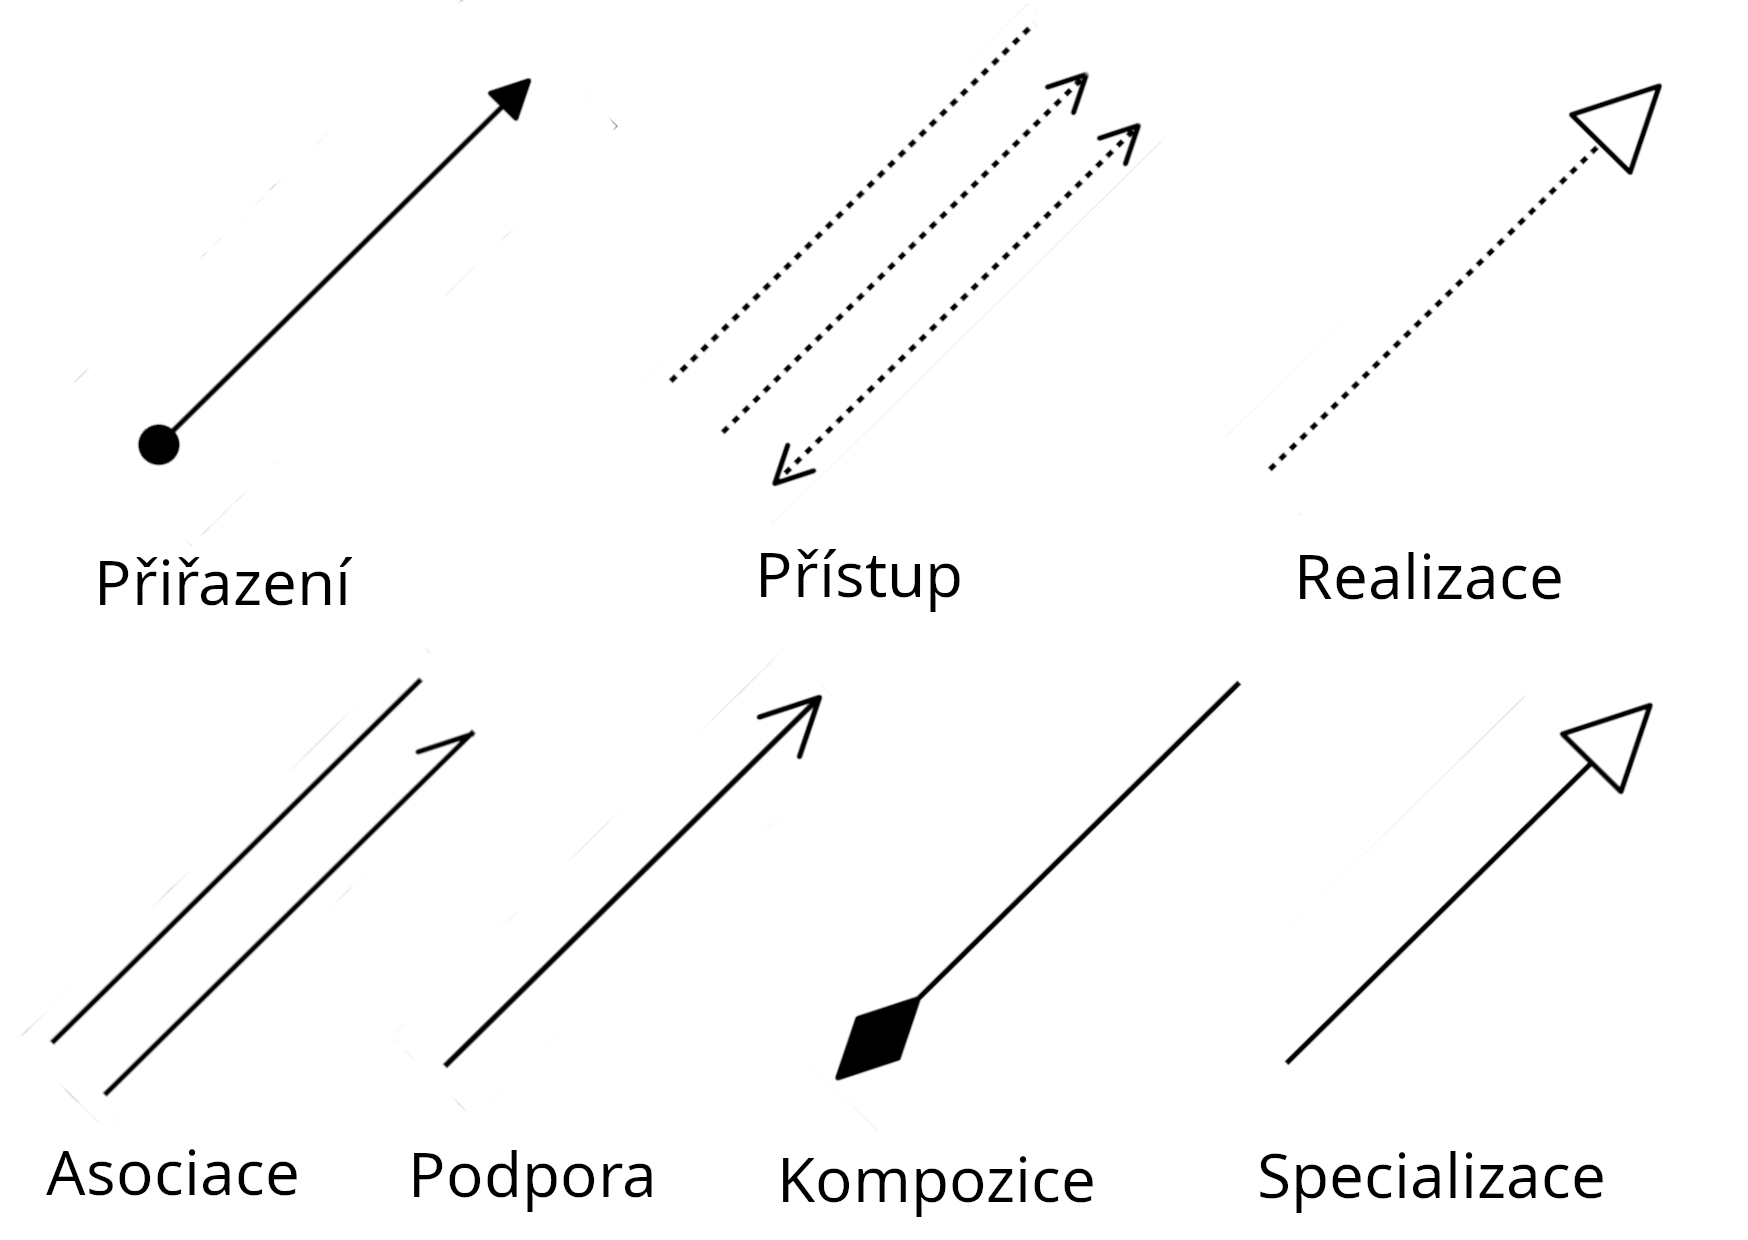
\includegraphics[width=0.8\textwidth]{img/relationships}

  \scriptsize \textit{Zdroj:} Vlastní zpracování na základě specifikace jazyka ArchiMate 3.2 \parencite{LanguageStructureArchiMate}
\end{figure}
